%%%%%%%%%%%%%%%%%%%%%%%%%%%%%%%%%%%%%%%%%%%%%%%%%%%%%%%%%%%%%
\subsubsection{数据准备与预处理}

问题1 的输入数据为附件1（10\degree 入射角）和附件2（15\degree 入射角），每条附件包含两列：波数 $\sigma$（cm$^{-1}$）和对应的反射率 $R$（\%）。数据预处理遵循"条纹即信号、禁止平滑"原则：

\textbf{P1 体检级清洗：} 检查波数轴均匀性，间隔变异系数 $<0.07\%$，确认无缺失值或跳变。波数范围约为 600--4000\,cm$^{-1}$。

\textbf{P2 剩余射线带剔除：} SiC 在 $\sigma<1100$\,cm$^{-1}$ 区间存在强烈的剩余射线带（Reststrahlen band），其反射率由晶格振动主导，不满足外延层干涉的简化条件。数据实验（EXP-5）确认该区域条纹不可靠，予以剔除。条纹区取 $\sigma\geq1100$\,cm$^{-1}$。

\textbf{P3 背景扣除：} 反射率谱可分解为缓变背景与周期条纹分量。背景由 7 阶多项式（poly7）对非振荡成分拟合得到，扣除后得到条纹分量 $F(\sigma)$ 用于后续分析。背景方案经三方案对比（poly7、频域高通、ALS 稳健基线），频域高通因 Gibbs 振铃导致条纹幅度畸变 709\% 触发红线出局，poly7 以零伪峰、跨角度极差最小定稿。

\textbf{噪声估计：} 背景扣除后，条纹分量的相邻点差分给出噪声稳健估计 $\hat{\sigma}_{\text{noise}}\approx0.012\%$（10\degree 和 15\degree 分别为 0.0117\%、0.0118\%）。该噪声水平极低，为后续残差诊断提供了参考基准。

\subsubsection{模型建立}

\textbf{步骤1：物理设置与记号。}

考虑三层介质结构：空气（$n_0=1$）/ 外延层（折射率 $n_1$，厚度 $d$）/ 重掺衬底（光学厚半空间）。平面波以入射角 $\theta$ 从空气射入，在外延层内的折射角 $\theta_1$ 由 Snell 定律给出：
\begin{equation}
    n_1\sin\theta_1 = \sin\theta
\end{equation}

给定波数 $\sigma$（cm$^{-1}$），真空中的相位随传播距离线性积累。

\textbf{步骤2：双光束复振幅叠加。}

空气/外延层界面的 Fresnel 振幅反射系数（近法线标量形式）为：
\begin{equation}
    r_{01} = \frac{1 - n_1\cos\theta_1}{1 + n_1\cos\theta_1}
\end{equation}
因 $n_1$ 为实数，$r_{01}$ 为实数。

衬底界面的反射具有复数特征：重掺衬底中自由载流子吸收使其反射系数为复数。在 v1.0 模型中，将其写作幅值-相位形式：
\begin{equation}
    r_{12}(\sigma) = \rho_{12} \cdot e^{i\varphi_{12}}
\end{equation}
其中 $\rho_{12}$ 为反射幅值，$\varphi_{12}$ 为有效常数相位（数据实验 EXP-1 证实自由拟合 $\varphi_{12}$ 跨角度稳定，差仅 0.025 rad，且 RMSE 显著优于固定 0 或 $\pi$）。

第二束光（经衬底界面反射后透出表面）相对于第一束光（表面直接反射）的相位差为：
\begin{equation}
    \Delta\varphi(\sigma) = 4\pi\,n_1\,d\,\cos\theta_1\cdot\sigma + \varphi_{12} = 2\pi\,p\,\sigma + \varphi_{12}
\end{equation}
其中 $p = 2n_1d\cos\theta_1$ 为往返光程（OPD），因子 4 来源于"往返各一次穿越外延层"（历史稿曾漏因子 2，实验纠正）。

双光束合成的反射场为：
\begin{equation}
    \frac{E_r}{E_0} = r_{01} + \rho_{12}\,e^{i\Delta\varphi(\sigma)}
\end{equation}

\textbf{步骤3：反射率谱与厚度的显式关系。}

由式(5)取模平方，得反射率谱：
\begin{equation}
    R(\sigma) = r_{01}^2 + \rho_{12}^2 + 2r_{01}\rho_{12}\cos(2\pi p\sigma + \varphi_{12})
\end{equation}

即"常数背景 $+$ 余弦条纹"：条纹幅度 $A=2|r_{01}\rho_{12}|$，条纹角频率 $2\pi p$，条纹周期（波数域）$\Delta\sigma = 1/p = 1/(2n_1d\cos\theta_1)$。

\textbf{步骤4：条纹级数与厚度确定原理。}

余弦条纹的极值条件为 $\cos(\cdot)=\pm1$，即：
\begin{equation}
    2\pi p\sigma_m + \varphi_{12} = m\pi, \quad m = 0, \pm1, \pm2, \ldots
\end{equation}

整理得条纹级数与波数的线性关系：
\begin{equation}
    m = 4n_1d\cos\theta_1\cdot\sigma_m + \frac{\varphi_{12}}{\pi}
\end{equation}

令斜率 $k = 4n_1d\cos\theta_1$，截距 $c = \varphi_{12}/\pi$，则：
\begin{equation}
    d = \frac{k}{4n_1\cos\theta_1}
\end{equation}

\textbf{可解性与唯一性讨论：}

（1）$d$ 与 $\varphi_{12}$ 通过"斜率 $+$ 截距"分离，要求极值级数覆盖至少 2 个条纹——本题可用条纹约 11.6 个，充分满足。

（2）极值序列 max/min 起始奇偶造成 $\varphi_{12}$ 的 mod-$\pi$ 简并（$\varphi_{12}$ 与 $\varphi_{12}+\pi$ 对应相同的极值位置但奇偶互换），需由全谱拟合或条纹幅度符号消除。

（3）$n_1$ 与 $d$ 在相位中仅以乘积 $n_1d$ 出现，双角度 $\cos\theta_1$ 差异仅 0.28\% 提供极弱辨识力——$n_1$ 取文献值，其偏差计入系统误差。数据实验（EXP-2）证实参数化色散与 $d$ 简并不可辨识（$n$ 估计值撞物理下界 2.30，$\sigma$ 估计值 13 无意义）。

（4）周期跳变（周跳）风险：极值回归存在多假设周期竞争，需在 GB/T 物理窗 $[3,200]\,\mu$m 内取 top-5 候选周期，全谱模型裁决最小 $\chi^2$ 者胜出。

\textbf{步骤5：模型参数定稿。}

四项物理设定经数据实验拍板（EXP-1$\sim$4，判据先行、选择-验证分离），定稿参数如表\ref{tab:model_params}所示。

\begin{table}[H]
  \centering
  \caption{双光束模型（v1.0）定稿参数}
  \label{tab:model_params}
  \small
  \begin{tabular}{p{1.8cm}p{2.8cm}p{3.8cm}p{4.2cm}}
    \toprule
    参数 & 取值 & 来源 & 确认方式 \\
    \midrule
    $n_1$ & 2.55（常数） & 文献红外值（Goldberg 2001）& EXP-2：参数化色散不可辨识 \\
    $\varphi_{12}$ & $\approx-0.28\pi$（约$-50$\degree）& 自由拟合 & EXP-1/4：跨角度稳定互证 \\
    $\rho_{12}$ & $\approx0.165$ & 自由拟合 & EXP-4 \\
    偏振 & 标量（不分 s/p）& s/p 差 $<3\%$ & EXP-3：四设定统计不可区分 \\
    衬底界面 & 常数反射率+常数相位 & Drude 自由拟合不可辨识 & EXP-4 \\
    \bottomrule
  \end{tabular}
\end{table}

\subsubsection{模型求解与结果}

图\ref{fig:fig2} 展示了 10\degree 和 15\degree 入射角下的实测反射率谱及多项式背景拟合。在 $\sigma<1100$\,cm$^{-1}$ 区域可见剩余射线带的强烈起伏，条纹区（$\sigma\geq1100$\,cm$^{-1}$）呈现规整的余弦振荡，且两角度条纹周期存在微小差异——这是厚度反演与双角度互证的物理基础。

\begin{figure}[H]
  \centering
  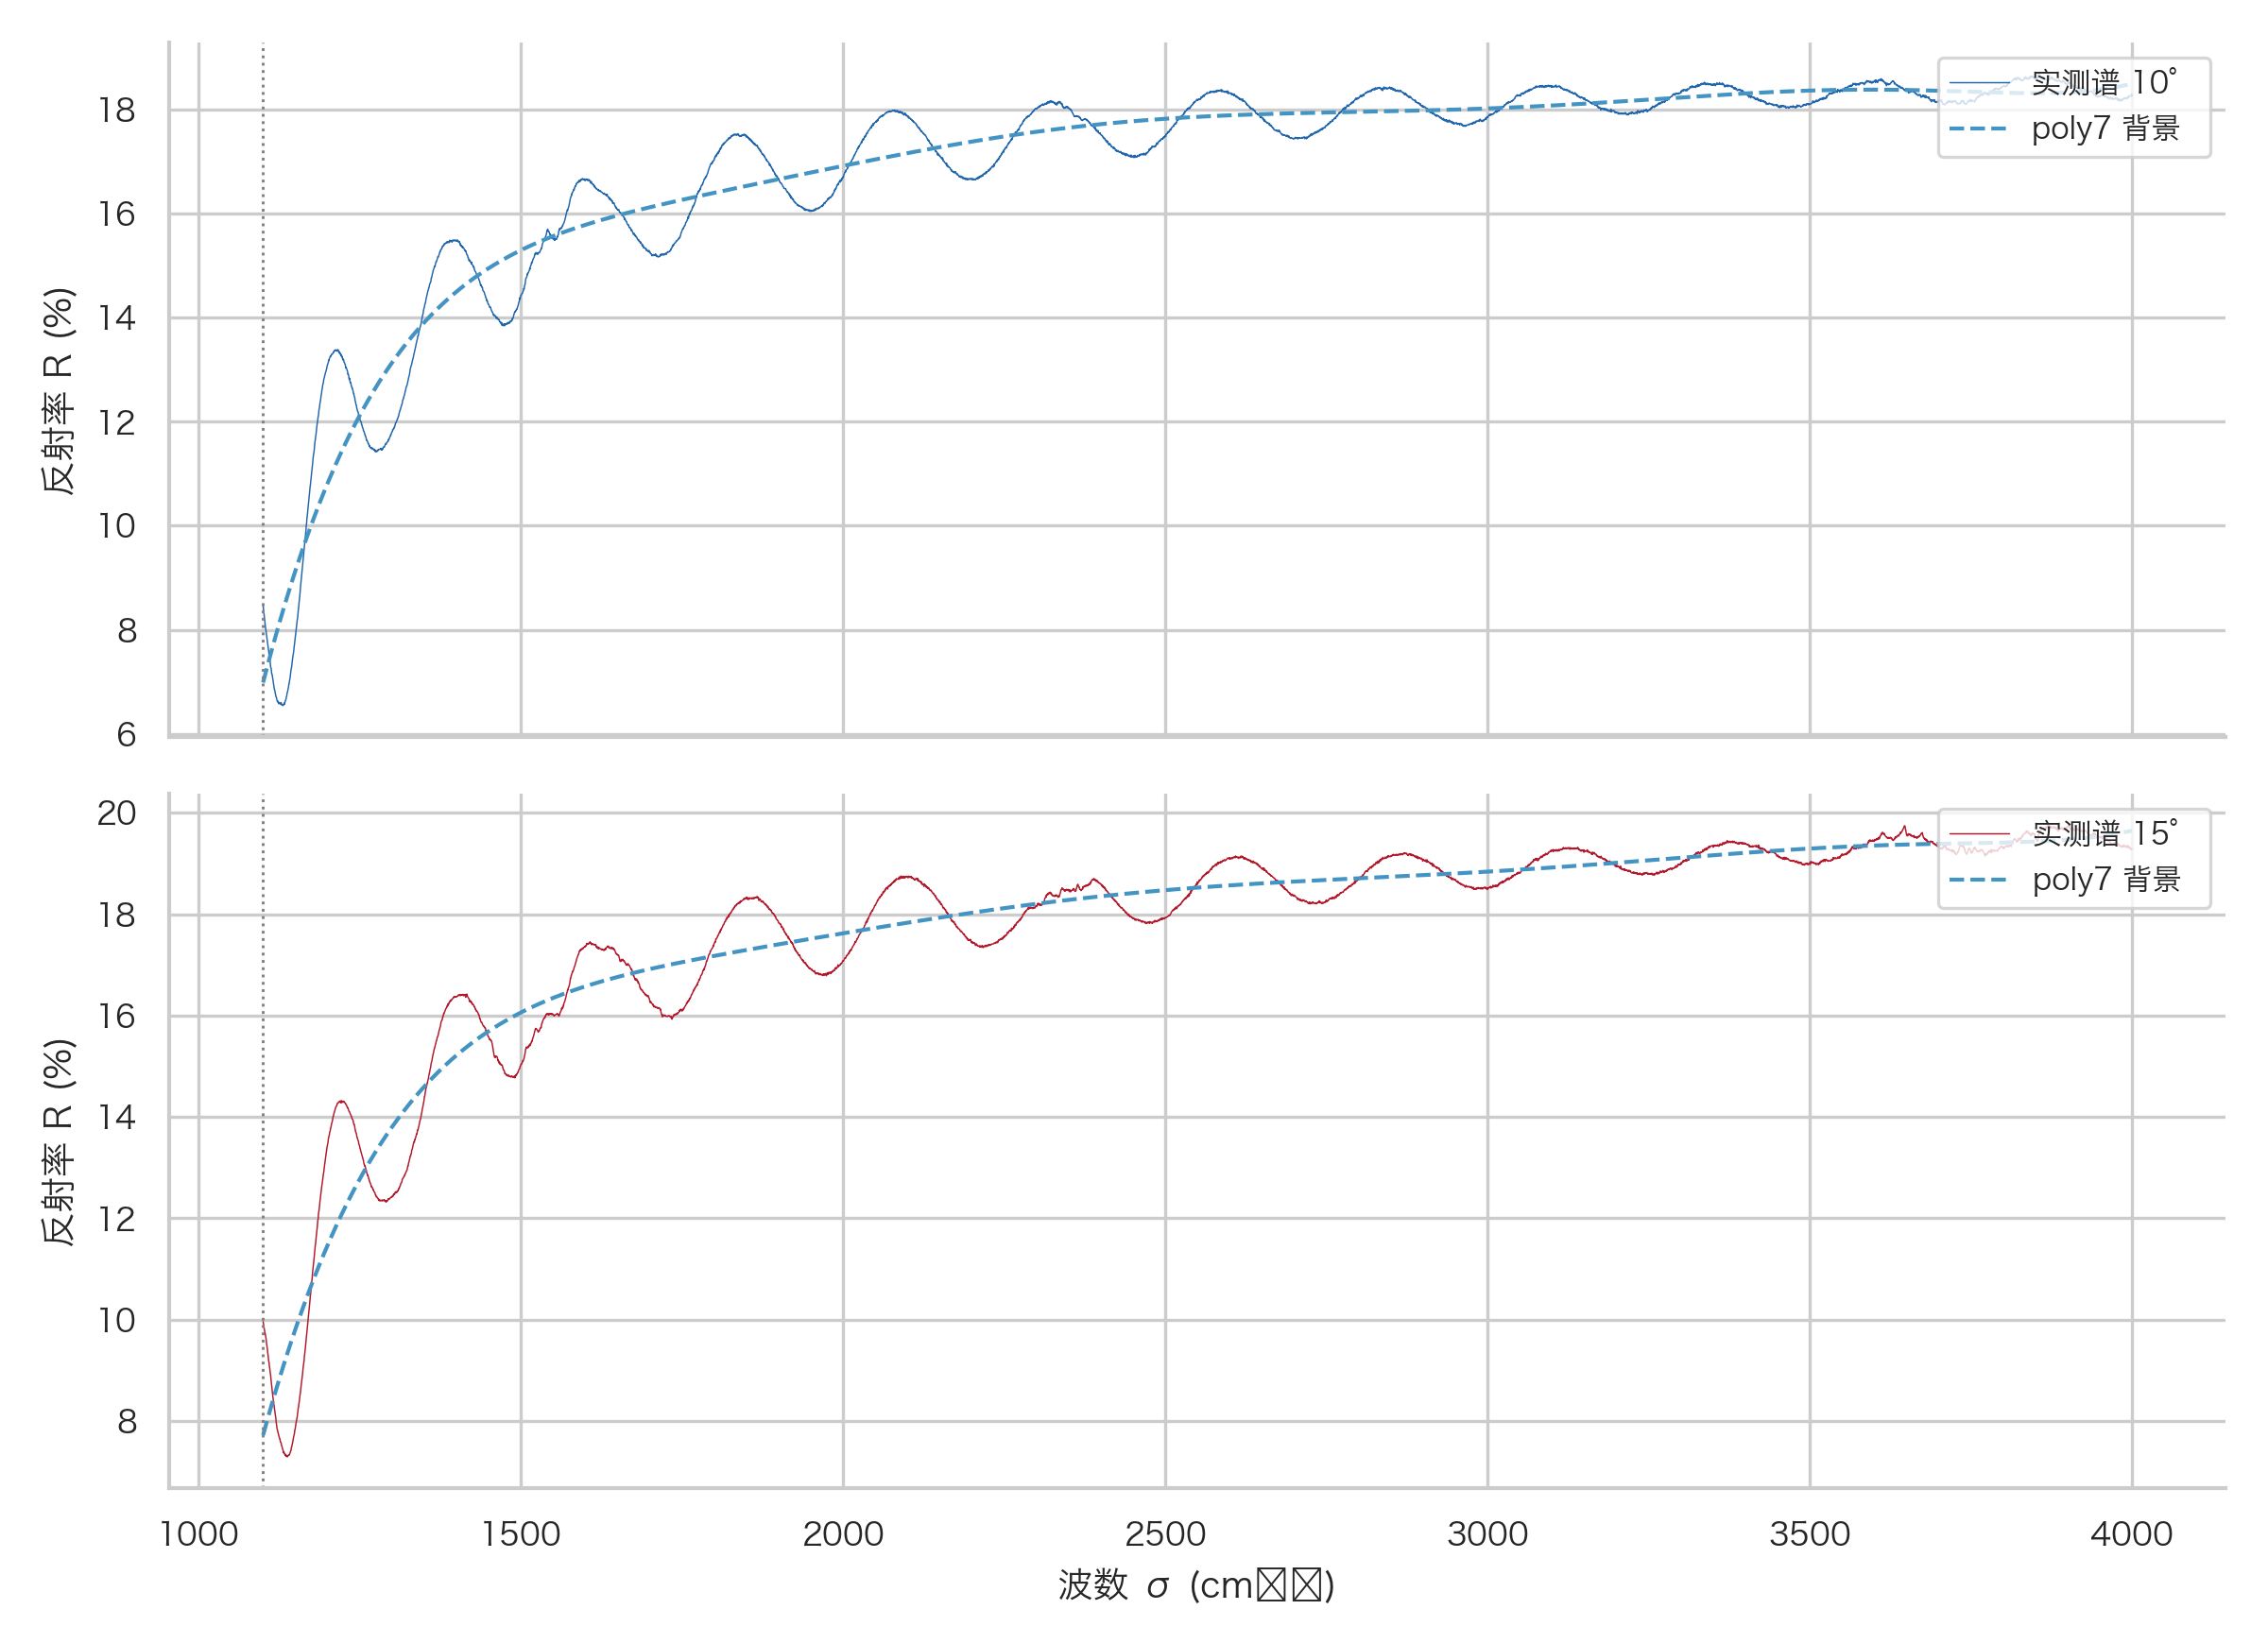
\includegraphics[width=0.9\textwidth]{../../03_结果与图表/最终图表/fig2_spectrum.png}
  \caption{实测反射率谱与多项式背景扣除（上：10\degree，下：15\degree）}
  \label{fig:fig2}
\end{figure}

根据式(8)，12 个极值点的线性回归给出 $k=2p$，进而由式(9)计算 $d$。极值回归法（E1）给出 $d_1=8.015$（10\degree）/ $7.801$（15\degree）$\mu$m。谱域 FFT 法（E2）和全谱拟合法（E3）的结果及三算法融合见问题2。

\begin{figure}[H]
  \centering
  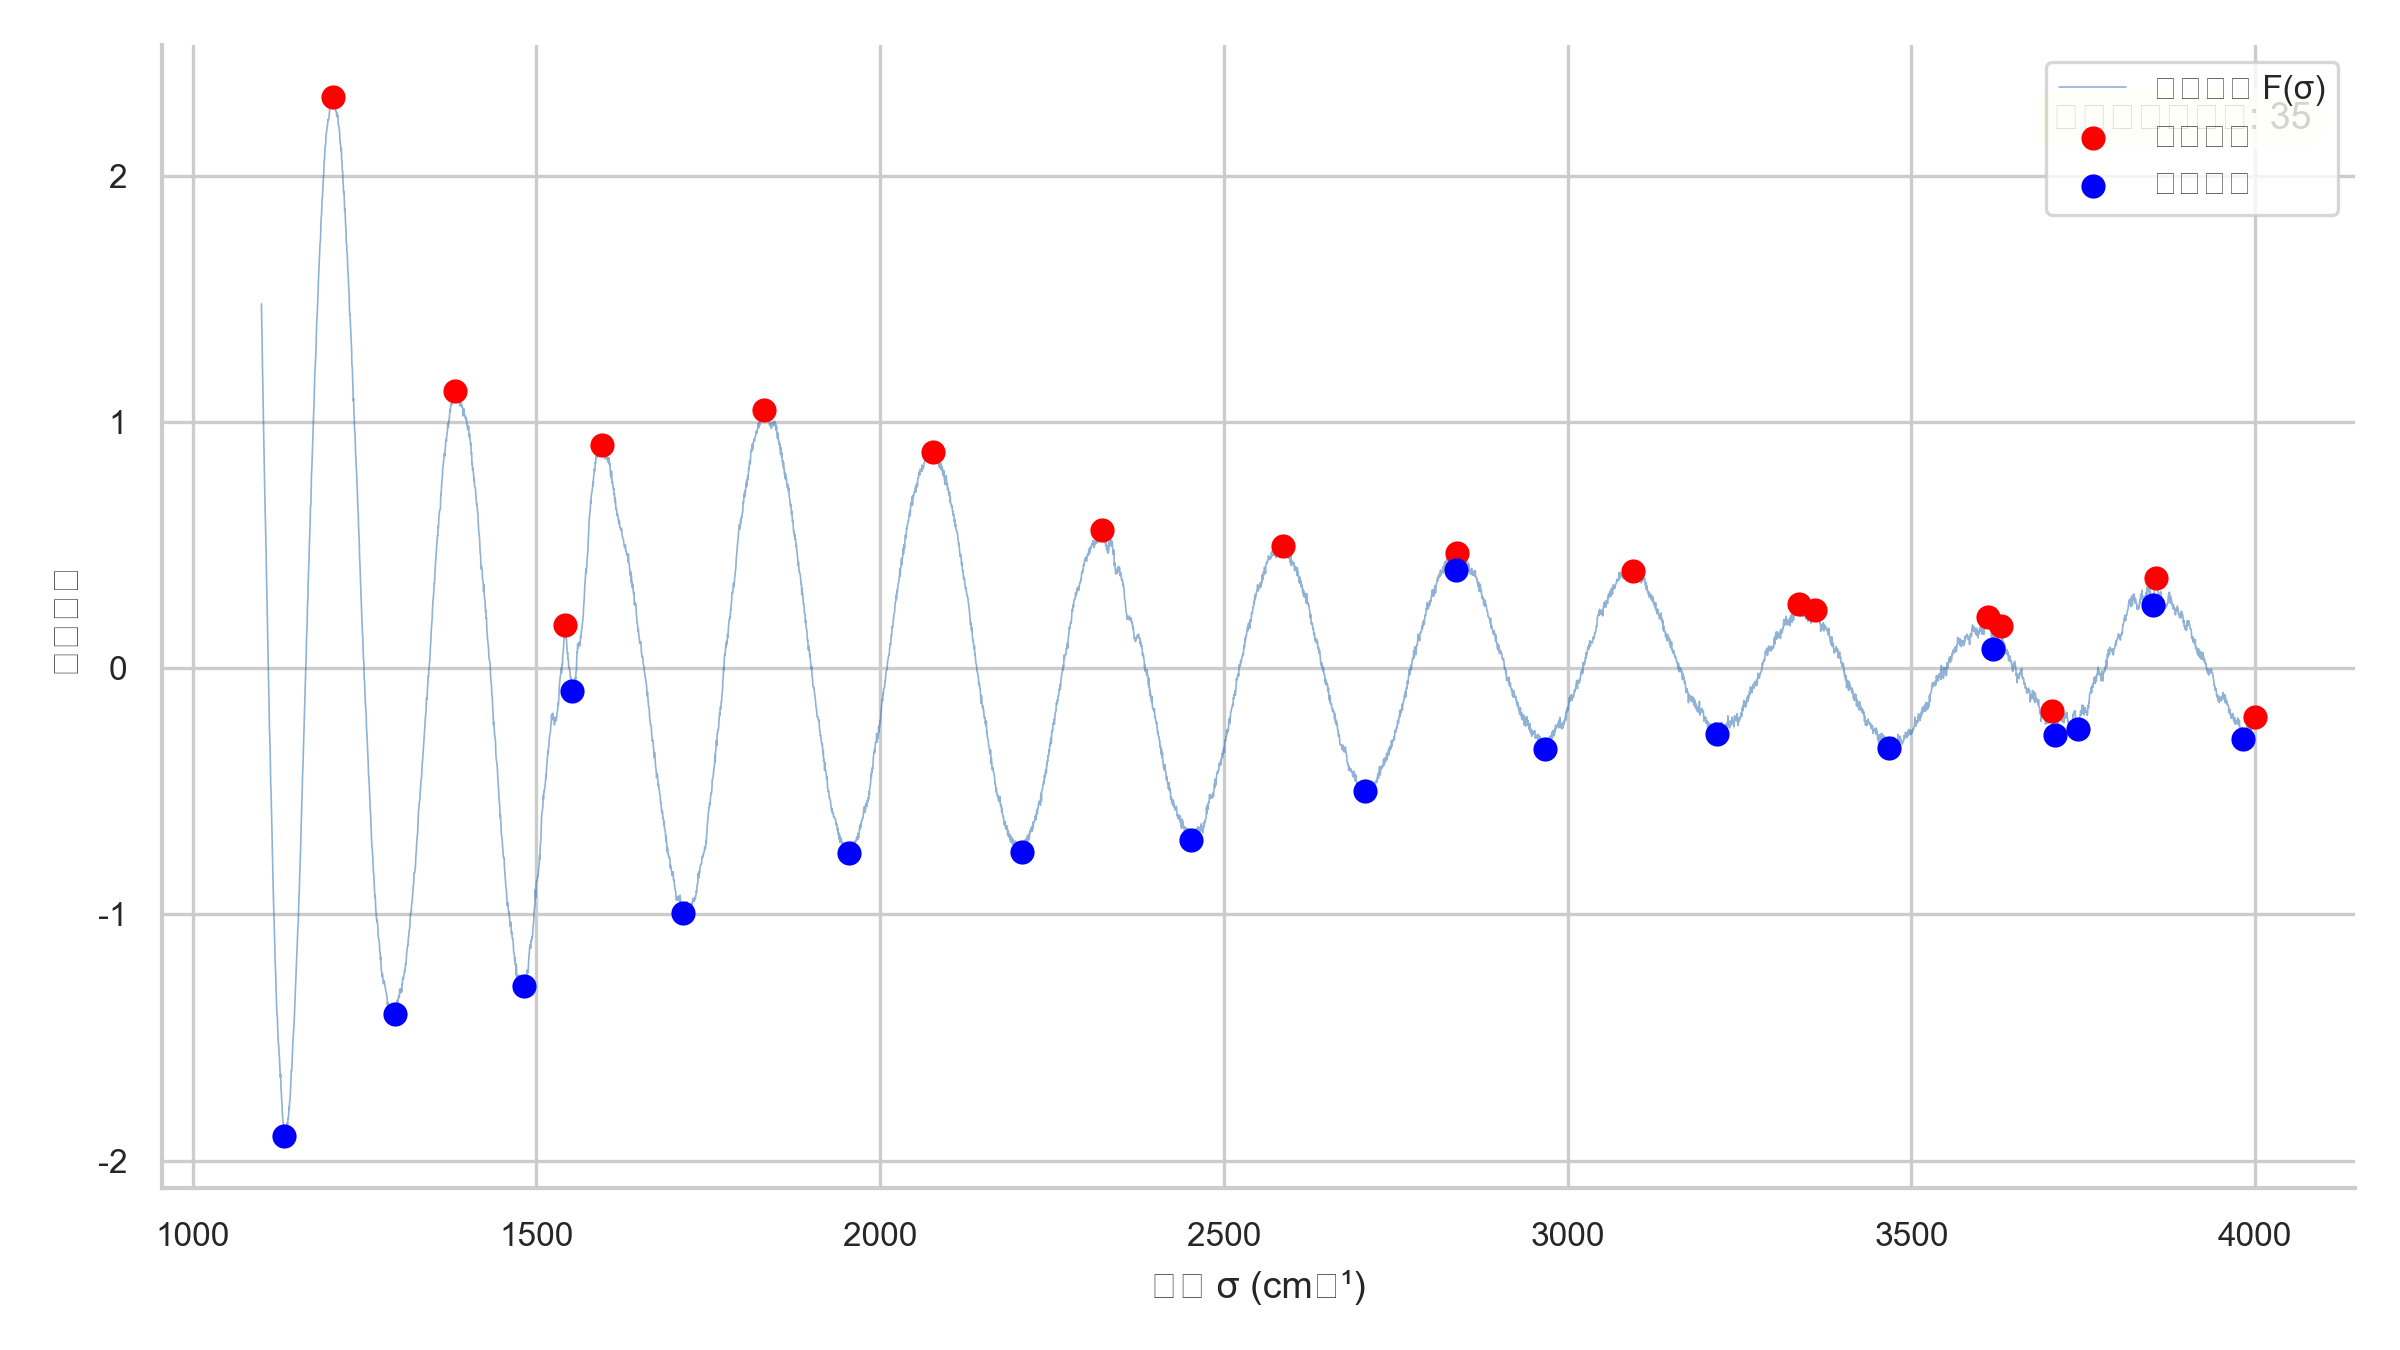
\includegraphics[width=0.88\textwidth]{../../03_结果与图表/最终图表/figA_extrema.png}
  \caption{条纹极值检测与分量可视化（10\degree）}
  \label{fig:extrema}
\end{figure}